\paragraph{Le package Sniffer}

La package Sniffer est le suivant. On y trouve les classes Adapter et RecyclerFragment. Ces classes seront détaillées ci-dessous.

\begin{minipage}
    {\linewidth}
    \centering
    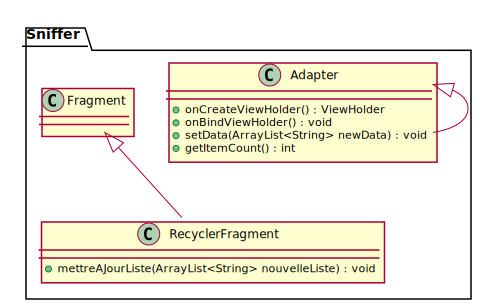
\includegraphics[width=0.30\linewidth]{../schemas/Conception_detaillee/classe_sniffer.pdf}
    \captionof{figure}{Diagramme du package Adapter}
\end{minipage}

\subparagraph{Philosophie de conception \newline} 

\medspace

La classe Adapter permet la mise en forme de RecyclerView. Celui-ci permet l'affichage d'un terminal. 

\subparagraph{Description structurelle \newline}

\medspace

\textbf{Attributs :}

N.A.

\textbf{Services offerts :}

\begin{itemize}
    \item \textbf{onCreateViewHolder() : ViewHolder } --- Opération qui crée l'instanciation du ViewHolder. 
    \item \textbf{onBindViewHolder() : void } --- Opération qui permet le binding du ViewHolder. 
    \item \textbf{setData(ArrayList<String> newData) : void } --- Opération qui permet l'ajout des données à afficher dans le RecyclerView.  
    \item \textbf{getItemCount() : int } --- Opération qui renvoie le nombre d'élément à répartir dans le RecyclerView. 
\end{itemize}



\paragraph{La classe RecyclerFragment}

\begin{minipage}
    {\linewidth}
    \centering
    \includegraphics[width=0.30\linewidth]{../schemas/Conception_detaillee/classe_snifferFragment.pdf}
    \captionof{figure}{Diagramme de la classe RecyclerFragment}
\end{minipage}

\subparagraph{Philosophie de conception \newline} 

\medspace

La classe RecyclerFragment permet la déclaration du fragment associé à la vue du sniffer CAN.  

\subparagraph{Description structurelle \newline}

\medspace

\textbf{Attributs :}

N.A.

\textbf{Services offerts :}

\begin{itemize}
    \item \textbf{mettreAJourListe(ArrayList<String> nouvelleListe) : void } --- Opération qui permet la mise à jour de la liste. Si la liste actuelle est la liste initiale, alors, elle est remplacée.  
\end{itemize}